\chapter{Problematyka prywatności i anonimowości w Internecie}
Technika, o której traktuje ta praca, jest ważnym tematem głównie dlatego, że
wykorzystanie jej do identyfikacji użytkowników ma istotne implikacje w obszarze
prywatności i anonimowości.

\section{Prywatność i anonimowość}
Prywatność internetowa to pewien podzbiór relacji pomiędzy gromadzeniem i
rozpowszechnianiem danych, technologią, społecznym oczekiwaniom wobec
prywatności i prawnymi oraz politycznym problemami orbitującymi wokół tych
zagadnień \cite{michael2013uberveillance}. W celach orientacyjnych stosowanym
uproszczeniem jest pogląd, że prywatność internetowa to możliwość zatrzymania
związanych z własną aktywnością danych dla siebie. Anonimowością jest zatem
sytuacja, w której przekazywanie takich danych jest zablokowane.

Prywatność i anonimowość użytkowników Internetu stała się zagadnieniem jeszcze
przed nadejściem ery Internetu \cite{david1965some}, pozwalając na koniec lat
dziewięćdziesiątych na zaognienie dyskusji, która trwa do dzisiaj. Użytkownicy
Internetu mają różne oczekiwania wobec poziomu ich prywatności w sieci. Mniej
wyczuleni na punkcie prywatności użytkownicy są w stanie pójść na pewny
kompromis pomiędzy wykorzystaniem ich danych a oferowanym na tej podstawie
potencjalnym usprawnieniem ich doświadczeń w Internecie (na przykład na
konkretnych stronach internetowych, w kontekście sieci reklamowych lub w innych
szerszych, kontekstach). Akceptują oni ryzyko zbyt szczegółowego profilowania,
potencjalnych naruszeń prywatności i inwigilacji. Inni użytkownicy dążą (mniej
lub bardziej) do utrzymania anonimowości takiej, jaka panowała w Internecie na
początku jego istnienia \cite[s. 54--69]{snowden2019pamiec}.

\subsection{Łączenie danych}
Istnieją firmy specjalizujące się w pozyskiwaniu, kupowaniu i przetwarzaniu
danych użytkowników w różnych celach (zwykle reklamowych). Nie wszystkie firmy
rynku danych przetwarzają dane w sposób naruszający prywatność użytkowników, ale
techniki takie jak łączenie danych z różnych źródeł (bez uprzedniej
anonimizacji) mogą lub będą prowadzić do nadużyć.

Bardzo sławny przypadek firmy Cambridge Analytica, która tworzyła profile
psychologiczne użytkowników i używała ich do manipulacji opinią publiczną za
pomocą mediów społecznościowych to jeden z przykładów firmy, która łącząc dane,
poważnie naruszyła prywatność użytkowników (m.in. Facebooka).

Istnieje wiele różnych dróg, dzięki którym w Internecie i w świecie rzeczywistym
użytkownicy będą nieświadomie profilowani lub inwigilowani, a łączenie danych z
różnych źródeł istotnie poprawi dokładność obrazu użytkownika. Jedną z takich
dróg jest używanie stron internetowych będących częścią większej sieci
reklamowej, która łączy dane na przykład z portali \emph{social media}, wyników
wyszukiwań, wysyłanych formularzy, a nawet z takich źródeł jak systemów
automatycznego wykrywania twarzy w sklepach stacjonarnych. Niektóre informacje,
które można wnioskować po automatycznym przetworzeniu to orientacja seksualna,
poglądy polityczne i religijne, rasa, historia użycia substancji
psychoaktywnych, estymowany iloraz inteligencji czy osobowość
\cite{kosinski2013private}.

\subsection{Czy prywatność jest nam potrzebna?}
Ochrona prywatności ma swoich przeciwników i zwolenników. ,,nie obchodzi mnie
prywatność, bo nie mam nic do ukrycia'' to argument przytaczany przez
przeciwników ochrony prywatności. Jedną z ważnych osób, które opowiedziały się
niegdyś za taką argumentacją, jest Eric Schmidt, były CEO firmy Google. Istnieje
silna polaryzacja pomiędzy przeciwnikami i zwolennikami ochrony prywatności. W
swojej książce autobiograficznej Edward Snowden (słynny amerykański
\emph{whistleblower}) stwierdził, że ,,oświadczyć, że nie obchodzi cię
prywatność, bo nie masz nic do ukrycia, to mniej więcej to samo, co oświadczyć,
że nie obchodzi cię wolność słowa, ponieważ nie masz nic do powiedzenia''
\cite{snowden2019pamiec}. Bruce Schneier, amerykański kryptograf i ekspert w
dziedzinie bezpieczeństwa komputerowego podsumowuje, że zbyt wiele osób myśli o
tym argumencie jak o wyborze pomiędzy bezpieczeństwem a prywatnością.
,,Prawdziwym wyborem jest wybór pomiędzy wolnością a kontrolą''
\cite{schneier2006eternal}. Prawo do prywatności zawiera się w Powszechnej
Deklaracji Praw Człowieka \cite{united1949universal}.

\section{Metody identyfikacji użytkowników}
Tak ja zauważono wcześniej w niniejszej pracy---wraz z komercjalizacją Internetu
powstał i ewoluował szereg różnych metod identyfikacji urządzeń, przeglądarek i
tym samym użytkowników. Istnieją różne zastosowania identyfikacji, ale jednym z
najbardziej powszechnie omawianych (i kontrowersyjnych) jest śledzenie
użytkowników (formalnie: łączenie ze sobą wielu wizyt jednego użytkownika na tej
samej platformie) \cite[s. 3]{al2020too}.

Warto także zauważyć, że \emph{fingerprinting} przeglądarek internetowych to
jedna z dróg identyfikacji urządzeń podłączonych do Internetu. Jest ona jednak
na tyle reprezentatywna, że często mówi się o \emph{fingerprintingu} urządzeń
jako \emph{fingerprintingu} przeglądarek. Dzieje się tak, ponieważ dzisiejsze
przeglądarki internetowe podczas interakcji z serwerami WWW mogą aktywnie lub
pasywnie przekazywać zestaw danych na tyle szeroki \cite{eckersley2010unique},
że zawiera on w sobie \emph{fingerprint} urządzenia, na którym działa
przeglądarka. Przeważający ogrom aktywności użytkowników wokół ,,przeglądania''
Internetu i wiele danych ,,oferowanych'' przez przeglądarki internetowe
naturalnie sprawia, że wysiłki identyfikujące użytkowników rozważane są głównie
w kontekście tychże. Niniejsza praca stara się zapewnić pewien (choć często
niewidoczny) podział. W kolejnym rozdziale niniejszej pracy omówiony jest także
\emph{fingerprinting} urządzeń podłączonych do Internetu, kiedy niemożliwe jest
wykorzystanie do celów identyfikacyjnych przeglądarki internetowej użytkownika.

Identyfikacja użytkowników nie zawsze jest także synonimem z identyfikacją
urządzeń czy przeglądarek, ale odsetek przypadków, kiedy w dzisiejszym świecie
więcej niż jedna osoba korzysta z np. jednej przeglądarki internetowej, wydaje
się stosunkowo niski. Powodem dla takiej estymacji jest fakt, iż wspomniane
przeglądarki, które posiadają istotny ułamek udziałów w rynku przeglądarek
internetowych, posiadają mechanizmy pozwalające na ich jednoznaczną
personalizację (parowanie z personalnym kontem Google w przeglądarce Google
Chrome, integracja przeglądarki Safari z ekosystemem firmy Apple, parowanie z
personalnym kontem Firefox w przeglądarce Firefox itd.). Co więcej, jeden
użytkownik może korzystać z wielu przeglądarek, co utrudnia jednoznaczną
identyfikację, ale nie czyni jej niemożliwą. Istnieją bowiem metody
\emph{fingerprintingu} urządzeń i przeglądarek pozwalające na identyfikację
użytkowników pomiędzy przeglądarkami internetowymi zainstalowanymi na tym samym
urządzeniu.

Gdyby podsumować metody identyfikacji użytkowników w dzisiejszym Internecie to
ich niedługa lista prezentowałaby się następująco:
\begin{itemize}
	\item Użycie \emph{cookies} (w szczególności \emph{third-party cookies});
	\item Użycie \emph{supercookies};
	\item Użycie \emph{fingerprintingu}.
\end{itemize}

Oczywiście nic nie stoi na przeszkodzie, aby każda z tych metod była używana w
połączeniu z innymi.

\section{Zagrożenia związane z fingerprintingiem}
Al-Fannah i Mitchell \cite[s. 1]{al2020too} konstatują, że identyfikacja za
pomocą \emph{fingerprintingu} jest znacznie trwalsza niż ta bazująca na
\emph{cookies}, praktycznie bez możliwości kontroli przez użytkowników i
nietrywialna do wykrycia. Istnieją zatem przynajmniej trzy powody, dla których
\emph{fingerprinting} stanowi istotnie większe zagrożenie dla prywatności
użytkowników (większe niż wszystkie dotychczasowe):
\begin{itemize}
	\item Na tę chwilę nie są znane proste sposoby, aby z całkowitą pewnością
	      wykryć, że dana platforma lub strona internetowa używa
	      \emph{fingerprintingu};
	\item Użytkownicy mogą kontrolować moc śledzenia za pomocą \emph{cookies},
	      regularnie usuwając je lub całkowicie blokując. Jak zostało
	      nadmienione wcześniej, istnieją także regulacje prawne dotyczące
	      użycia \emph{cookies}. Nie ma jednak żadnych porównywalnych, równie
	      prostych do użycia technik kontroli \emph{fingerprintingu};
	\item \emph{Fingerprinting} (w przeciwieństwie do \emph{cookies}) nie polega
	      na jednej, konkretnej właściwości HTTP. \emph{Fingerprinting} bazuje
	      na wielu technologiach, aby zbierać różne informacje o właściwościach
	      i konfiguracji przeglądarki lub systemu operacyjnego. Każda z tych
	      informacji to szansa, aby zastosować \emph{fingerprinting}.
\end{itemize}

Co więcej, \emph{fingerprinting} może być użyty do tworzenia
\emph{supercookies}, czyli specjalnych \emph{cookies}, które po usunięciu mogą
zostać ponownie utworzone, jeśli ta sama przeglądarka zostanie wykryta przez
użycie \emph{fingerprintingu} \cite[s. 2]{al2020too}.

\section{Możliwości ochrony przed fingerprintingiem}
Autorzy monografii dotyczącej metod kontroli i ochrony przed
\emph{fingerprintingiem} wyróżniają dwa typy rozwiązań ochrony przed
\emph{fingerprintingiem}: możliwe do zastosowania przez użytkowników i takie,
które powinny zostać zaimplementowane przez autorów oprogramowania
\cite{al2020too}.

\subsection{Perspektywa użytkownika}
Kontrola i ochrona, którą mogą zastosować użytkownicy to wybór przeglądarki i
jej konfiguracja (np. Firefox posiada pewne ustawienia dotyczące ograniczania
\emph{fingerprintingu}---Rys. 2) lub instalacja dodatkowych rozszerzeń, które
blokują lub ograniczają \emph{fingerprinting}, blokując JavaScript, fałszując
atrybuty lub blokując przesyłanie ich zawartości. Niestety każdy z wymienionych
sposobów wiąże się obecnie z istotną degradacją jakości przeglądania Internetu.
Przy wyborze aktualnie prawdopodobnie najbardziej skupionej na prywatności
przeglądarki Tor możemy spotkać się z wieloma ostrzeżeniami. Jest to na przykład
prośba o niemaksymalizowanie okna przeglądania, aby zapobiec efektywnemu
używaniu atrybutu rozdzielczości ekranu podczas ewentualnego
\emph{fingerprintingu}. Używając wyżej wymienionych sposobów, musimy także
liczyć się z tym, że wiele stron internetowych może po prostu przestać działać.
Niektóre z rozszerzeń, chociaż często ograniczonych przez to na jak wiele
pozwalają autorzy oprogramowania, mogą paradoksalnie przyczynić się do
dokładniejszego \emph{fingerprintingu}. Omawiany \emph{fingerprintability
	paradox} nazywa sytuację, w której próby ograniczenia \emph{fingerprintingu}
nieintencjonalnie tworzą nowe źródło danych, których można użyć w trakcie
\emph{fingerprintingu}. Problem widoczny jest szczególnie, wtedy kiedy danego
rozszerzenia używa niewielu użytkowników. Niektóre z rozszerzeń mogą także
fałszować atrybuty w taki sposób, że są one bardzo rzadkie lub wręcz
nierealistyczne. Taka sytuacja sprzyja unikalnej identyfikacji. Paradoks był
szeroko omawiany w środowisku naukowym \cite{eckersley2010unique,torres2015fp}.
Autorzy monografii podkreślają też, że nie ma obecnie żadnych poważnych badań
dotyczących efektywności istniejących rozszerzeń mających zapobiegać przed
\emph{fingerprintingiem}.

\begin{figure}
	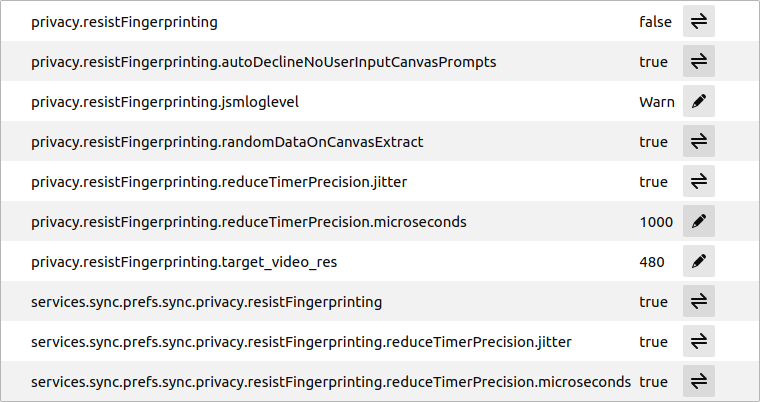
\includegraphics[width=\textwidth,keepaspectratio]{img/02}
	\source{about:config}
	\caption{Opcje ograniczające \emph{fingerprinting} w Firefox 79.0}
\end{figure}

\subsection{Perspektywa twórców oprogramowania}
Zakres działań, które mogą podjąć twórcy przeglądarek internetowych, jest
znacznie szerszy niż to, czego mogą dokonać sami użytkownicy. Aktualnie
wszystkie główne przeglądarki internetowe różnią się w stopniu dokładności
\emph{fingerprintu}, jaki może zostać utworzony na podstawie danych przez nie
dostępnych. Redukcja informacji lub całkowite wyeliminowanie niektórych
nagłówków zapytań HTTP, jednorodność w implementacji, kontekstowy dostęp i
wycofywanie starych oraz niepotrzebnych funkcji z API przeglądarek to tylko
niektóre z kroków, jakie mogłoby podjąć konsorcjum przeglądarek, aby drastycznie
zwiększyć ich prywatność. Istnieje szereg rekomendacji dotyczący tej kwestii
\cite{cooper2013privacy,doty2014fingerprinting,eckersley2010unique,nikiforakis2014workings}.
Warto także zauważyć, że praktycznie żaden z kroków możliwych do podjęcia od tej
strony nie wiąże się z utratą jakości przeglądania/funkcjonowania stron
internetowych. Niestety niektórzy producenci przeglądarek mogą być niechętni do
podejmowania kroków mających na celu ograniczyć \emph{fingerprinting}. Powodem
tej sytuacji może być fakt, że czerpią oni korzyści finansowe z serwisów
internetowych korzystających z tej metody identyfikacji \cite[s. 13]{al2020too}.

\subsection{Czy da się skutecznie zapobiec fingerprintingowi?}
Al-Fannah i Mitchell podsumowują \cite[s. 18]{al2020too}, że wydaje się
nieprawdopodobne, abyśmy w najbliższym czasie przestali słyszeć o
\emph{fingerprintingu}. Badania pokazują, że jego użycie ciągle rośnie.
Identyfikacja za pomocą \emph{fingerprintingu} ma także inne zastosowania niż
śledzenie użytkowników (patrz 2.5), więc całkowite pozbycie się go bez
zaproponowania innej alternatywy wydaje się niemożliwe do osiągnięcia w
praktyce. Jako alternatywę autorzy proponują \emph{Unique Browser Identifier}
(UBI). Sami jednak podkreślają paradoksalną naturę proponowanego rozwiązania i
obawy przed jego potencjalnie niepoprawnymi implementacjami \cite[s.
16]{al2020too}. Biorąc pod uwagę brak stanowczych kroków ze strony producentów
przeglądarek i w przypadku braku innych alternatyw przewiduje się, że efektywne
zapobieżenie \emph{fingerprintingowi} będzie w najbliższej przyszłości
niemożliwe. Mając na uwadze to, jak dużym jest zagrożeniem dla prywatności
użytkowników, bezsprzecznie jest to ważny przedmiot przyszłych badań.

\section{Inne zastosowania fingerprintingu}
Valentin Vasilyev, który zapoczątkował cieszący się dużą popularnością
otwartoźródłowy projekt
\textbf{fingerprintjs}\footnote{https://github.com/fingerprintjs/fingerprintjs2}
i jest obecnie współzałożycielem firmy
FingerprintJS\footnote{https://www.linkedin.com/in/valentin-vasilyev}, na jej
stronie internetowej\footnote{https://fingerprintjs.com} pokazuje, że
\emph{fingerprinting} posiada wiele innych, różnych zastosowań w ramach
identyfikacji użytkowników. Są to między innymi zastosowania dotyczące
wykrywania masowego i zautomatyzowanego tworzenia fałszywych kont oraz
fałszerstw (w kontekście transakcji elektronicznych) w serwisach internetowych.
Także firma Cloudflare zapobiega atakom na serwisy swoich klientów, korzystając
z techniki Google
Picasso\footnote{https://support.cloudflare.com/hc/en-us/articles/360045224651}
(\emph{fingerprinting} urządzeń i przeglądarek opracowany przez Google
\cite{45581}). \emph{Fingerprinting} może być zatem także czymś w rodzaju
drugiej warstwy uwierzytelniającej w serwisach internetowych.
